\documentclass[english,10pt,a4paper]{article}
\usepackage[T1]{fontenc}
\usepackage{babel}
\usepackage{fontawesome5}			% To add icons
\usepackage{xcolor}					% To add colors
\usepackage[scale=0.87]{geometry}	% To manage page margins
\usepackage{graphicx} 				% To add graphics
\usepackage[hidelinks]{hyperref}	% To add link
\usepackage{stix}
\usepackage{longtable}
\usepackage{fancyhdr}
\pagestyle{fancy}

% -------------------------------------------------------------------------------- %
% CV Colors...
% -------------------------------------------------------------------------------- %
\definecolor{CvColor}{RGB}{0, 147, 202}

% -------------------------------------------------------------------------------- %
% Footer and Header...
% -------------------------------------------------------------------------------- %

% clear existing header/footer entries
\fancyhf{} 
\renewcommand{\headrulewidth}{0pt}

% Place Page X of Y on the right-hand
% side of the footer
\fancyfoot[R]{\textcolor{CvColor}{\rule[.5\baselineskip]{\textwidth}{1pt}} Page \textbf{\thepage} \hspace{1pt}}

% -------------------------------------------------------------------------------- %
% Commands...
% -------------------------------------------------------------------------------- %

% To add level to skill...
\newcommand{\BasicLevel}{{\footnotesize (\textit{Foundation})}}
\newcommand{\MediumLevel}{{\footnotesize (\textit{Intermediate})}}

% To add education info in educational section...
\newcommand{\CvEducation}[2]{ {\small \textit{#1}: #2}}

% To add a bullet...
\newcommand{\CvBullet}{\hspace{0.05cm} \textcolor{CvColor}{$\bullet$} \hspace{0.05cm}}

% To design CV section...
\newcommand{\CvSection}[2]{\vspace{0.5cm}
	{\LARGE \textcolor{CvColor}{#1 \hspace{2pt} \textbf{#2}}} \\
	\textcolor{CvColor}{\rule[.5\baselineskip]{0.5\textwidth}{0.5pt}}}

% To design 'Time Range'...
\newcommand{\CvTimeRange}[2]{\textcolor{CvColor}{\textsc{#1 - #2}}}

% To design 'Date'...
\newcommand{\CvDate}[1]{\textcolor{CvColor}{{\textsc{#1}}}}

% To desing experience as block...
\newcommand{\FullBlock}{\textcolor{CvColor}{\mdlgblksquare}}
\newcommand{\EmptyBlock}{\textcolor{CvColor}{\square}}

% To customize "itemize" enviroment
\renewcommand{\labelitemi}{$\textcolor{CvColor}{\circ}$}
\renewcommand{\labelitemii}{$\textcolor{CvColor}{\bullet}$}

% -------------------------------------------------------------------------------- %
% Variables.
% -------------------------------------------------------------------------------- %

\def\SidebarHSize{3.5cm}
\def\BodyHSize{11cm}

% -------------------------------------------------------------------------------- %
% Longtable size (see documentation https://ctan.mirror.garr.it/mirrors/ctan/macros/latex/required/tools/longtable.pdf)
% -------------------------------------------------------------------------------- %

\setlength\LTpre{0.15cm}
\setlength\LTpost{0.15cm}

\begin{document}
	
	{\Huge \textcolor{CvColor!50}{\textbf{Andrea}} \textcolor{CvColor!80}{\scshape \textbf{Graziani}}} \hfill
	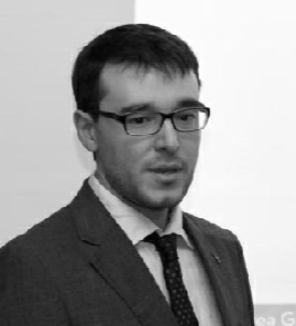
\includegraphics[width=8em]{./Images/Photo.png} \\
	\textcolor{CvColor}{\rule[.5\baselineskip]{\textwidth}{1pt}}
	
	% ================================================================================ %
	% Personal Data
	% ================================================================================ %
	
	\begin{tabular}{rlrl}
		\textsc{Place and Date of Birth:} & Italy, 27 August 1993 \CvBullet \hspace{0.05cm} \textsc{Age}: 29 & \textsc{\faGithub} & \href{https://github.com/AndreaG93}{\texttt{AndreaG93}} \\
		
		\textsc{Address:} & Viale S. Francesca Saverio Cabrini, 8 & \textsc{\faLinkedin} & \href{https://it.linkedin.com/in/andrea-graziani-5134b8256}{\texttt{andrea-graziani-5134b8256}} \\
		
		& 00077 Monte Compatri (RM), Italy & \faCar & Driving licence B \CvBullet Car available \\
		
		\textsc{Phone:} & +(39)~333~78~58~512 && \\
		\textsc{E-mail:} & \href{mailto:andrea.graziani.ing@outlook.com}{\texttt{andrea.graziani.ing@outlook.com}} && \\
		\textsc{Nationality}: & Italy
	\end{tabular}
	
	% ================================================================================ %
	% Education
	% ================================================================================ %
	\CvSection{\faGraduationCap}{Education}
	
	% -------------------------------------------------------------------------------- %
	% Master’s Degree
	% -------------------------------------------------------------------------------- %
	\begin{longtable}{p{\SidebarHSize}|p{\BodyHSize}}
		\CvTimeRange{2018}{2022} & \textbf{Master’s Degree}, Computer engineering \\
		& \textsc{Università degli Studi di ROMA ``Tor Vergata"} \\
		& \textsc{LM-32 - 2nd level degree in Computer engineering}\\
		& \\
		& \CvEducation{Final degree mark}{\textbf{110/110 cum laude}} \\
		& \CvEducation{Dissertation/thesis title}{``A QoS-aware broker for multi-provider serverless applications"} \CvBullet \CvEducation{Thesis supervisor}{Valeria Cardellini} \\
		& \CvEducation{Age at graduation}{28} \CvBullet \CvEducation{Graduation date}{23/05/2022}	
	\end{longtable}
	
	% -------------------------------------------------------------------------------- %
	% Bachelor's degree
	% -------------------------------------------------------------------------------- %
	\begin{longtable}{p{\SidebarHSize}|p{\BodyHSize}}
		\CvTimeRange{2012}{2018} & \textbf{Bachelor's degree}, Computer engineering \\
		& \textsc{Università degli Studi di ROMA ``Tor Vergata"} \\
		& \textsc{L-8 - 1st level degree in Information technology}\\
		& \\
		& \CvEducation{Final degree mark}{\textbf{102/110 cum laude}} \\	
		& \CvEducation{Age at graduation}{25} \CvBullet \CvEducation{Graduation date}{26/10/2018}	
	\end{longtable}
		
	% -------------------------------------------------------------------------------- %
	% Diploma
	% -------------------------------------------------------------------------------- %
	\begin{longtable}{p{\SidebarHSize}|p{\BodyHSize}}
		\CvTimeRange{2008}{2012} & \textbf{Italian Secondary School Diploma}, Scientific Certificate \\
		& \textsc{Liceo Scientifico Statale Bruno Touschek} \\	
		& \\
		& \CvEducation{School-leaving examination mark}{\textbf{90/100}} \\
		& \CvEducation{Graduation date}{2012}	
	\end{longtable}

	% ================================================================================ %
	% Work Experience
	% ================================================================================ %
	\CvSection{\faBriefcase}{Work Experience}

	\begin{longtable}{p{\SidebarHSize}|p{\BodyHSize}}
		\CvTimeRange{June 2022}{Present} & \textbf{Software Engineer}, ALTEN Italia S.p.A. - Rome, Italy \\
		& \\
		& Acted as computer consultant for following companies: 
		  \begin{itemize}
			\item \textbf{ABB S.p.A.} - Rome, Italy \newline
			\textbf{(June 2022 - June 2023)} \newline
			To develop several web applications, acting as management software, used by some company departments in order to perform some task like data management, report extraction, scheduling activities and so on.
			\begin{itemize}
				\item Acted as software designer, developer, tester and coordinator of the projects.
				\item Performed requirements gathering and technical documentation.
				\item Handled production deployment, testing and technical support.
				\item Started initiatives aimed at improving software development process.
				\item Performed bug fixing.
			\end{itemize}
		\end{itemize} \\
		& \begin{itemize}
			\item \textbf{GF Machining Solutions S.p.A.} - Meyrin, Switzerland \newline
			\textbf{(June 2023 - Present)} \newline
			To develop a web application that allows users to setup, manage laser industrial machines for making metallurgical products.
			\begin{itemize}
				\item Acted as a developer.
				\item Updated technical documentation.
				\item Performed bug fixing.
			\end{itemize}
		\end{itemize}
	\end{longtable}
	
	% ================================================================================ %
	% Training
	% ================================================================================ %
	\CvSection{\faBook}{Training}
	
	\begin{longtable}{p{\SidebarHSize}|p{\BodyHSize}}
		\CvDate{September 2022} & \textbf{RabbitMQ usage in event driven architecture} \\
		& \textsc{Training course at ALTEN Italia S.p.A. (Rome, Italy)} \\
		& \\	
		& Introductory course on event-oriented architectures and how to configure and use a RabbitMQ cluster.
	\end{longtable}
	
	% ================================================================================ %
	% Language
	% ================================================================================ %
	\CvSection{\faLanguage}{Language}

	\begin{longtable}{p{\SidebarHSize}|p{\BodyHSize}}
		\CvDate{Mother tongue} & Italian \\
		& \\
		
		\CvDate{Foreign language(s)} & \begin{tabular}{c|c|c|c|c}
			\textbf{Language} & \textbf{Listening} & \textbf{Reading} & \textbf{Writing} & \textbf{Speaking} \\
			\hline 
			&&&&\\		
			English & \texttt{B1} & \texttt{B2} & \texttt{B2} & \texttt{B1} \\
		\end{tabular}
	\end{longtable} 
	
	% ================================================================================ %
	% Computer Skill
	% ================================================================================ %
	\CvSection{\faLaptop}{Computer Skills}

	% -------------------------------------------------------------------------------- %
	% Programming Languages / Markup Languages
	% -------------------------------------------------------------------------------- %
	
	\begin{longtable}{p{\SidebarHSize}p{\BodyHSize}}
		\CvDate{Languages} &  \begin{tabular}{lcr}
			\centering
			& \textbf{Experience} & \textbf{Experience Years} \\
			\hline
			&& \\
			\texttt{C} & $\FullBlock\FullBlock\FullBlock\EmptyBlock\EmptyBlock$ & 2 \\
			\texttt{C++} & $\FullBlock\EmptyBlock\EmptyBlock\EmptyBlock\EmptyBlock$ & 0.5 \\
			\texttt{C\#} & $\FullBlock\FullBlock\FullBlock\FullBlock\EmptyBlock$ & 1.5 \\
			\texttt{Java} & $\FullBlock\FullBlock\FullBlock\EmptyBlock\EmptyBlock$ & 2 \\
			\texttt{Go} & $\FullBlock\FullBlock\FullBlock\EmptyBlock\EmptyBlock$ & 1.5 \\
			\texttt{Python} & $\FullBlock\FullBlock\FullBlock\EmptyBlock\EmptyBlock$ & 1.5 \\
			\texttt{Assembly MIPS} & $\FullBlock\EmptyBlock\EmptyBlock\EmptyBlock\EmptyBlock$ & 0.5 \\
			\texttt{Assembly x86} & $\FullBlock\EmptyBlock\EmptyBlock\EmptyBlock\EmptyBlock$ & 0.5 \\
			\texttt{HTML} & $\FullBlock\FullBlock\FullBlock\EmptyBlock\EmptyBlock$ & 2 \\
			\texttt{CSS} & $\FullBlock\FullBlock\EmptyBlock\EmptyBlock\EmptyBlock$ & 0.5 \\
			\LaTeX & $\FullBlock\FullBlock\FullBlock\EmptyBlock\EmptyBlock$ & 5 \\
		\end{tabular}
	\end{longtable}
	
	% -------------------------------------------------------------------------------- %
	% Other
	% -------------------------------------------------------------------------------- %
	
	\begin{longtable}{p{\SidebarHSize}p{\BodyHSize}}
		\CvDate{Cloud} & Apache OpenWhisk \BasicLevel \CvBullet AWS EC2 \BasicLevel \CvBullet AWS Lambda  \BasicLevel \CvBullet AWS Step Functions \BasicLevel \CvBullet AWS CloudWatch \BasicLevel \CvBullet SonarQube \BasicLevel
	\end{longtable}
		
	\begin{longtable}{p{\SidebarHSize}p{\BodyHSize}}
		\CvDate{Build automation} & Maven \BasicLevel \CvBullet CMake \BasicLevel
	\end{longtable}
		
	\begin{longtable}{p{\SidebarHSize}p{\BodyHSize}}
		\CvDate{Databases} & Microsoft SQL Server \MediumLevel \CvBullet PostgreSQL \MediumLevel \CvBullet InfluxDB \BasicLevel \CvBullet Apache Cassandra \BasicLevel \CvBullet Apache Kakfa \BasicLevel \\
	\end{longtable}
	
	\begin{longtable}{p{\SidebarHSize}p{\BodyHSize}}
		\CvDate{ORM} & Entity Framework \MediumLevel \CvBullet Hibernate \BasicLevel
	\end{longtable}
	
	\begin{longtable}{p{\SidebarHSize}p{\BodyHSize}}
		\CvDate{OS} & Microsoft Windows \MediumLevel \CvBullet Kubuntu \MediumLevel \CvBullet KDE Neon \MediumLevel \CvBullet Manjaro \MediumLevel \CvBullet Arch Linux \MediumLevel \\
	\end{longtable}
	
	\begin{longtable}{p{\SidebarHSize}p{\BodyHSize}}
		\CvDate{Web Programming} & Blazor \MediumLevel \CvBullet JSP \BasicLevel \\
	\end{longtable}
	
	\begin{longtable}{p{\SidebarHSize}p{\BodyHSize}}
		\CvDate{IDE} & Android Studio \BasicLevel \CvBullet CLion \MediumLevel \CvBullet IntelliJ IDEA Community Edition \MediumLevel \CvBullet GoLand \MediumLevel \CvBullet PyCharm Community Edition \MediumLevel \CvBullet Visual Studio \MediumLevel \CvBullet Google Colaboratory (Colab) \BasicLevel \CvBullet \\
	\end{longtable}
	
	\begin{longtable}{p{\SidebarHSize}p{\BodyHSize}}
		\CvDate{DevOps} & Azure DevOps \BasicLevel \CvBullet JIRA Software \BasicLevel \CvBullet Travis CI \BasicLevel \\
	\end{longtable}
	
	\begin{longtable}{p{\SidebarHSize}p{\BodyHSize}}
		\CvDate{Testing} & JUnit \BasicLevel \CvBullet MSTest \BasicLevel \CvBullet Moq \BasicLevel \CvBullet Mockito \BasicLevel
	\end{longtable}
	
	\begin{longtable}{p{\SidebarHSize}p{\BodyHSize}}
		\CvDate{Others} & git \MediumLevel \CvBullet docker \BasicLevel \CvBullet Apache ZooKeeper \MediumLevel \CvBullet Valgrind \BasicLevel \CvBullet \texttt{lp\_solve} \BasicLevel \CvBullet  Gurobi \BasicLevel \CvBullet Some deep learning libraries (\texttt{TensorFlow} and \texttt{Keras}) \BasicLevel \CvBullet RabbitMQ \BasicLevel \\
	\end{longtable}
	
\end{document}










